%!TEX root = ../chapter3.tex
%******************************
%	 Introduction 
%*****************************

\section{Introduction}

Gametogenesis describes the process that generates haploid gametes, which carry one copy of the individuals DNA. 
Sexual reproduction requires the fusion of two gametes, from each of the opposite sexes, to drive evolution and adaptation \citep{McDonald2016}. 
Spermatogenesis, the male version of gametogenesis, is a tightly regulated developmental process that ends in the generation of mature sperm. During spermatogenesis, spermatogonial stem cells undergo a unidirectional differentiation programme to form mature spermatozoa. 
This process occurs in the epithelium of seminiferous tubules in the testis \textbf{(Fig.~\ref{fig3:cell_staging}B)} and is tightly coordinated to ensure the continuous and life-long production of mature sperm cells. 
In the mouse, the first step involves spermatogonial differentiation to form pre-leptotene spermatocytes \citep{Oakberg1971, DeRooij1973, DeRooij2000}. 
Pre-leptotene spermatocytes then commit to meiosis, a cell division programme that consists of two consecutive cell divisions to produce haploid cells. 
To accommodate homologous recombination between sister chromatids and chromosome synapsis \citep{Marston2004}, prophase of meiosis I is extremely prolonged, lasting several days in males. 
It can be divided into four substages: leptonema, zygonema, pachynema and diplonema. 
Following the two consecutive cell divisions, haploid cells known as round spermatids undergo a complex differentiation programme called spermiogenesis to form mature spermatozoa \citep{Oakberg1956}. \\

Spermatogenesis takes place in a highly orchestrated fashion, with tubules periodically cycling through twelve epithelial stages defined by the combination of germ cells present (see \textbf{Fig.~\ref{fig3:cell_staging}B} and \citep{Oakberg1956}). 
The completion of one cycle takes 8.6 days in the mouse, and the overall differentiation process from spermatogonia to mature spermatozoa requires approximately 35 days \citep{Oakberg1956a}. 
Thus, three to four generations of germ cells are present within a tubule at any given time. 
In adults, each tubule resides in a different cycle stage meaning that at any given time point a continuum of germ cell types is present in the testis \textbf{(Fig.~\ref{fig3:cell_staging})}. 
The continuity of this differentiation process and the gradual transitions between spermatogenic cell types have made the isolation and thus the molecular characterisation of individual sub-stages during spermatogenesis difficult.

\newpage

\begin{figure}[!h]
\centering
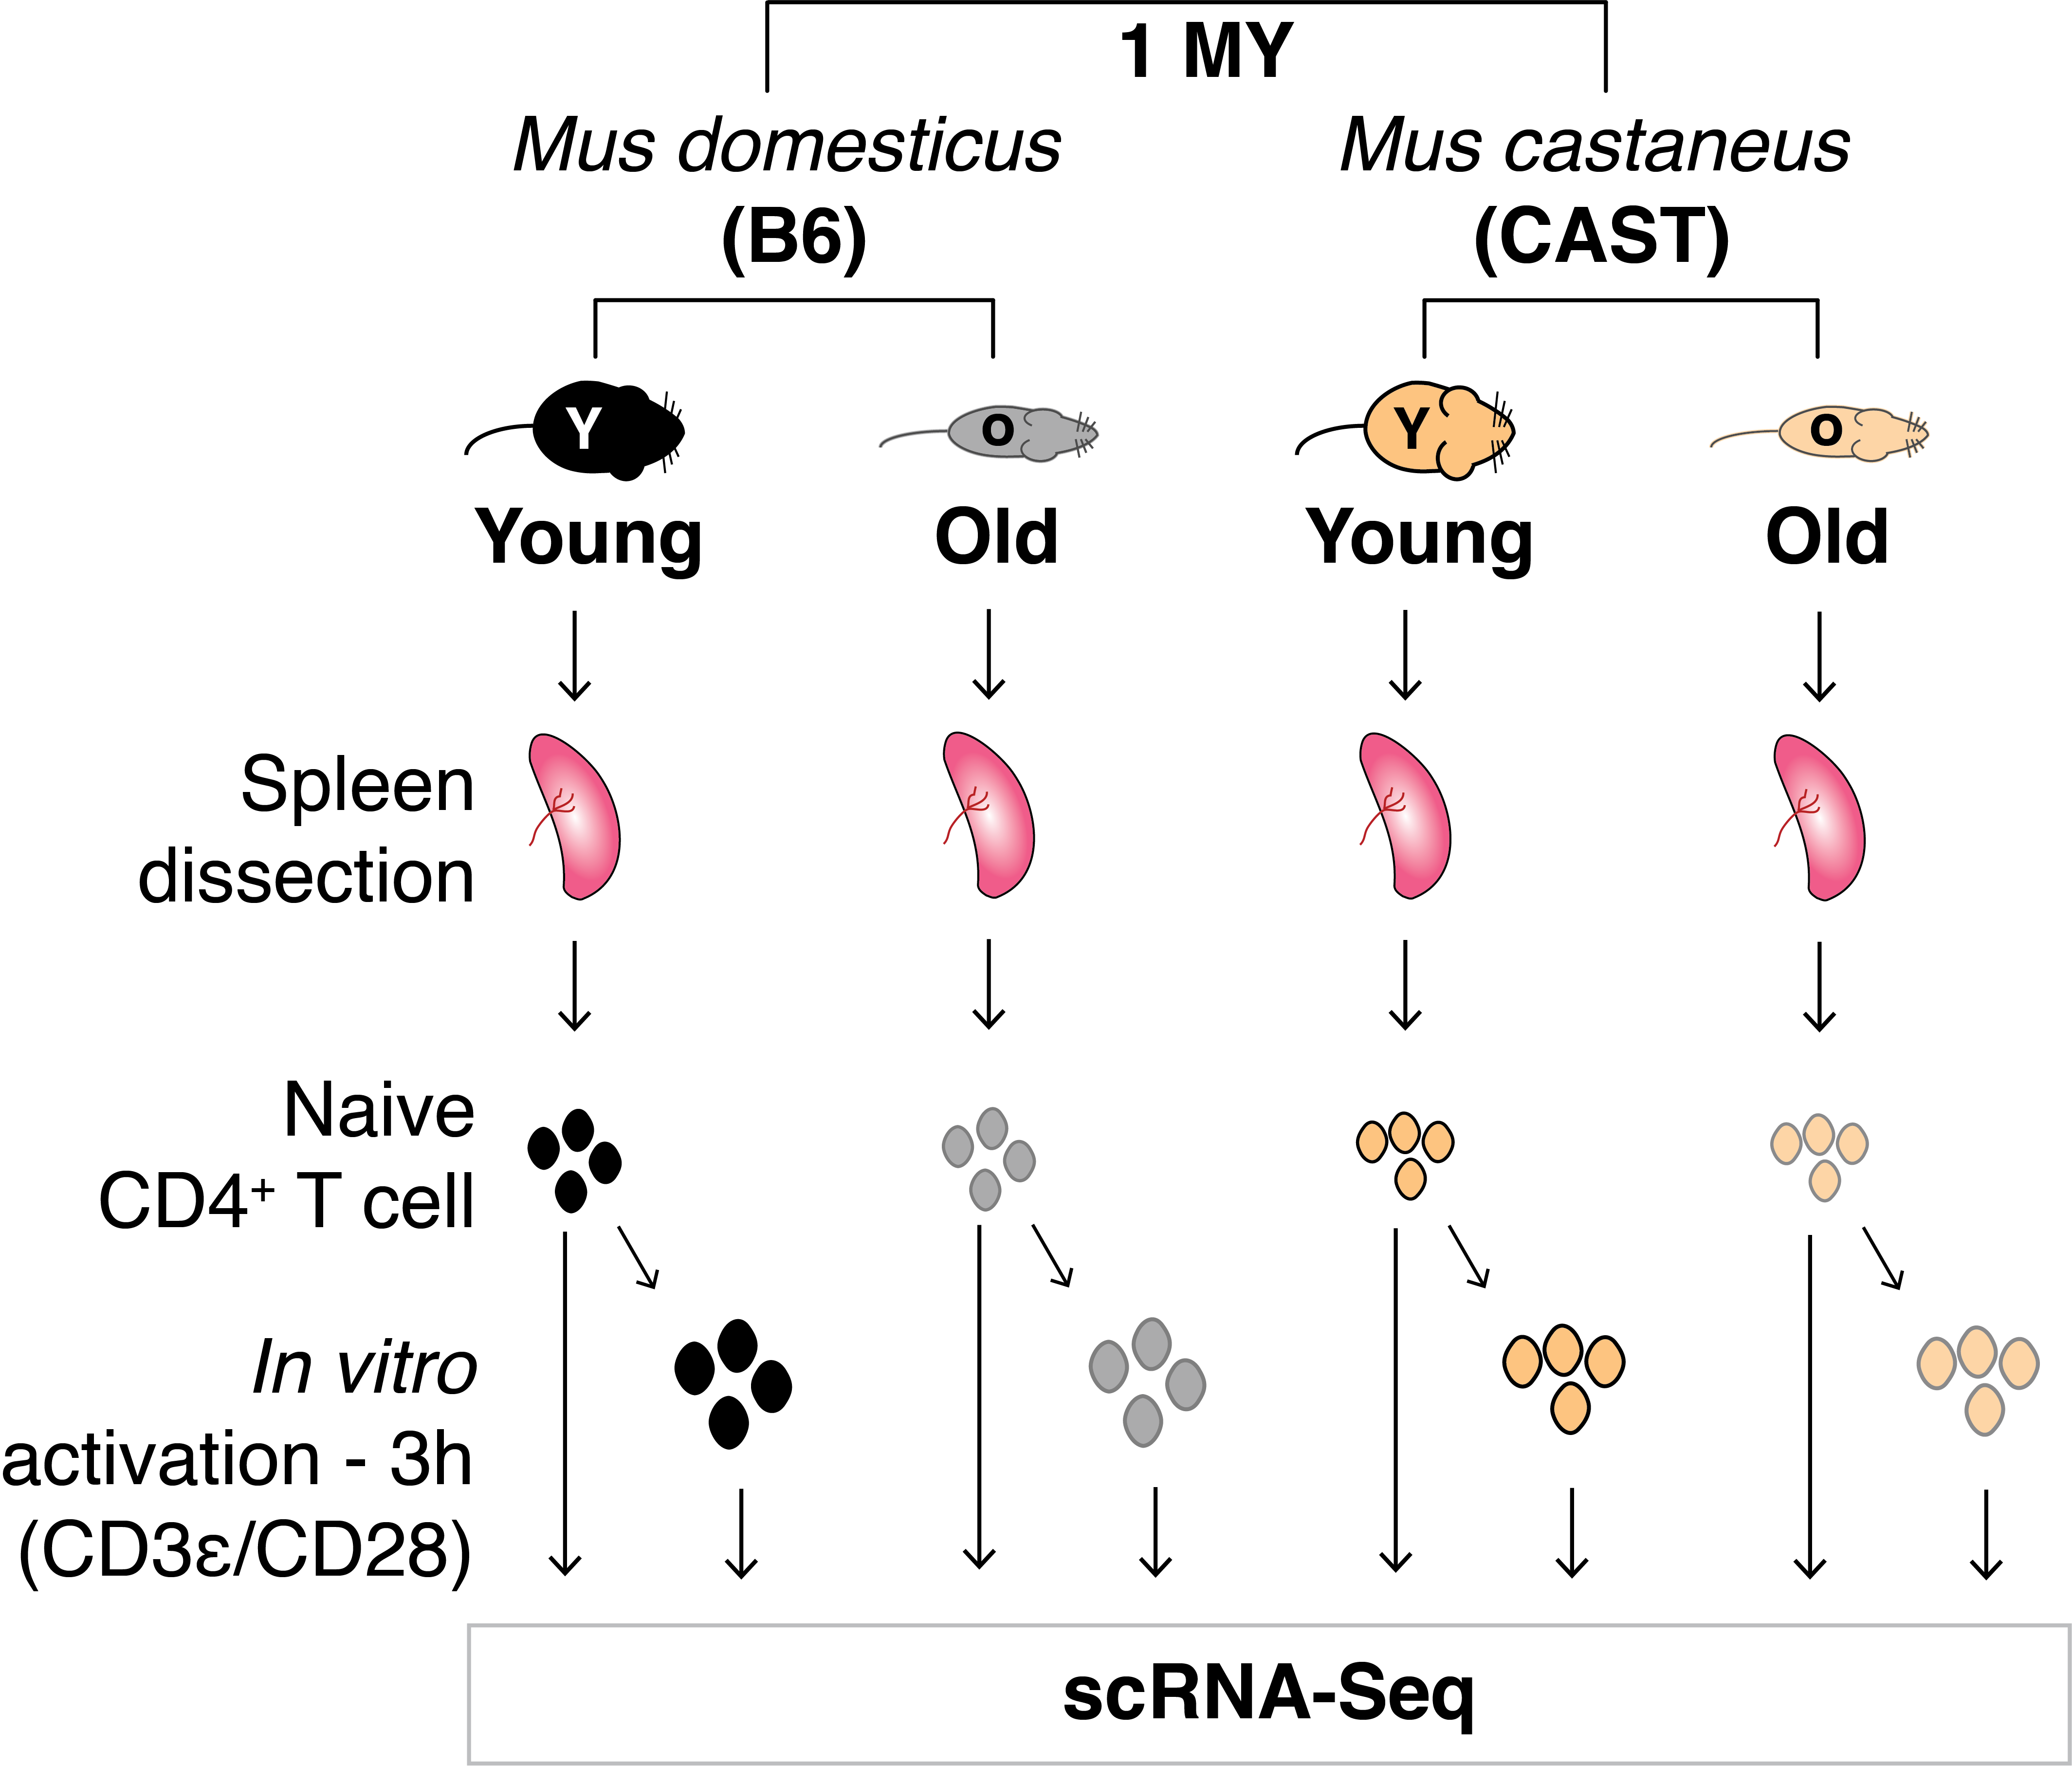
\includegraphics[width=0.9\textwidth]{Fig_1.png}
\caption[Staging of the testicular seminiferous epithelium]{\textbf{Staging of the testicular seminiferous epithelium.}\\
\textbf{(A)} Periodic Acid Schiff (PAS)-stained testis cross-section showing a number of seminiferous tubules at different epithelial stages (displayed as Roman numerals). Within each tubule, the inset circle refers to the corresponding section in (B). 
Scale bar represents 100 \textmu{}m, 
\textbf{(B)} Schematic representation of the 12 stages of the seminiferous epithelium in mice. 
The colour gradient within the circle indicates the differentiation path of germ cells with the layers corresponding to individual cycles of the epithelium. 
The circle is divided into 12 section, each corresponding to one epithelial stage displaying the characteristic germ cells. 
Within each section, cells are positioned across the different layers according to their emergence during consecutive cycles, each being 8.6 days apart with more mature cells moving towards the centre, 
\textbf{(C)} Higher magnification of two tubules depicted in (A). The PAS-stained cross-sections show tubules in Stage VII and Stage X, with the different cell layers indicated by coloured lines. 
Stage VII tubules contain 4 different layers with germ cells from different generations that are approximately 8.6 days apart, whereas Stage X tubules only contain three layers. 
Cell types are labelled as: \gls{A}, \gls{In}, \gls{B}, \gls{Pl}, \gls{LS}, \gls{ZS}, \gls{PS}, \gls{DS}, \gls{M}, \gls{S}: round spermatids stages 1-8 and elongating spermatids stages 9-16, \gls{SG}, \gls{SC}.}
\label{fig3:cell_staging}
\end{figure}

\newpage

To fully elucidate the molecular genetics of germ cell development, it is crucial to sample the full spectrum of germ cells present in testes of adult animals. 
For this purpose, we employed an unbiased droplet-based scRNA-Seq approach using the 10X Genomics\texttrademark{} platform. 
We used the transcriptomic profiles of thousands of single germ cells to characterise the complex transcriptional dynamics of spermatogenesis at a high-resolution. 
To confidently identify and label cell populations throughout the developmental trajectory, we profiled cells from juvenile testes during the first wave of spermatogenesis. 
In juveniles, spermatogenesis has only progressed to a defined developmental stage, which therefore allowed us to unambiguously identify the most mature cell type by comparison with adult. 
The correct labelling of cell types was then used to dissect differentiation processes such as meiosis and spermiogenesis. 
Furthermore, juvenile samples were enriched for spermatogonia, which allowed us to characterise spermatogonial differentiation. 
Another major developmental process during spermatogenesis is the inactivation and reactivation of the X chromosome, which is subject to transcriptional silencing as a consequence of asynapsis \citep{Turner2007}. 
By combining bulk and single-cell RNA-Seq approaches with chromatin profiling, we identified that \textit{de novo} activated X-linked genes carry distinct chromatin signatures with high levels of repressive H3K9me3 in spermatocytes. \\

Finally, after fully characterising the transcriptional changes during spermatogenesis, I used the regression model presented in the previous chapter to study changes in transcriptional variability over the differentiation time course. 
To this end, I generated \emph{post hoc} posterior distributions of linear regression coefficients to statistically test whether individual genes increase or decrease in variability. 
Furthermore, the clustering of variability profiles showed that rapid transcriptional changes during differentiation can cause peaks in such variability profiles.
